\documentclass[a4paper,11pt,oneside]{article}
\usepackage[pdftex]{graphicx}
\usepackage[utf8]{inputenc}
\usepackage[spanish]{babel}
\usepackage{fancyhdr}
\usepackage[usenames,dvipsnames]{color}
\usepackage{colortbl}
\usepackage{tabularx}
\usepackage{hyperref}
\usepackage{pdfpages}
\usepackage{lscape}


\setlength{\headheight}{15.2pt}
\pagestyle{fancy}

\lhead{\nouppercase{\leftmark}}
\chead{}
\rhead{}

\hypersetup{
colorlinks,
citecolor=black,
filecolor=black,
linkcolor=black,
urlcolor=black
}

\setlength{\parskip}{6pt}

\begin{document}

%%%% Title Page %%%%%

%\pagenumbering{alph}

\begin{titlepage}
\begin{center}

% Upper part of the page

\includegraphics[width=0.2\textwidth]{img/logo-uclm.png}\\[1cm]
\textsc{\LARGE Escuela Superior de Informática}\\[0.5cm]
\textsc{\Large Universidad de Castilla -- La Mancha}\\[2.5cm]

% Title
{\LARGE Práctica 1}\\[0.5cm]
\rule{\linewidth}{0.5mm}\\[0.4cm]
{\huge \textbf{Tres en Raya Definitivo Web}}\\
\rule{\linewidth}{0.5mm}\\[0.4cm]

% Authors
\begin{minipage}{0.5\textwidth}
\begin{flushleft}
\large
\hspace{1cm}\textbf{\emph{Autores}}\\
Marchán Loro, Javier\\
Peralta López, Ángel\\
Pérez Pascual, Rubén\\
Ruedas García, Antonio\\
\end{flushleft}
\end{minipage}
\vfill

% Bottom of the page
\begin{minipage}{\textwidth}
\large
\begin{tabular}{rl}
\textbf{Asignatura}: & Ingeniería del Software II\\
\textbf{Titulación}: & Ingeniería Informática\\
\textbf{Fecha}: & \today
\end{tabular}
\end{minipage}

\end{center}
\end{titlepage}

%%%% end Title Page %%%%%

\pagenumbering{roman}
\setcounter{page}{1}

\tableofcontents
\clearpage

\pagenumbering{arabic}
\setcounter{page}{1}

\clearpage
\section{Introducción}

Este documento describe el análisis, desarrollo e implementación llevados a cabo para obtener
el juego \textbf{Tres en Raya Definitivo} \footnote{Este documento no explica las reglas del juego}.

Se trata de una aplicación cliente-servidor para escritorio que se comunica a través de RMI.
El lenguaje utilizado para la implementación ha sido Java.

Este documento pretende que el lector obtenga una idea clara de la composición del sistema, para ello
se ha dividido en distintas secciones. En primer lugar los requisitos funcionales ayudan a entender el objetivo
buscado. La arquitectura del sistema junto con los casos de uso son las secciones más importantes, ya
que ayudarán al lector a hacerse una imagen mental, a alto nivel, del sistema desarrollado.

El resto de secciones profundizan en el conocimiento del sistema.

\clearpage


\section{Arquitectura del sistema} 

En la Figura \ref{arq_sistema} se muestra una visión de la arquitectura del sistema. Se
trata de una arquitectura cliente-servidor a través de RMI. El cliente usa
un proxy para comunicarse con el servidor y éste conoce un proxy de cada
cliente con el que se comunica. Toda la logica del juego reside en el cliente.

 \begin{figure}[h]
 \centering
 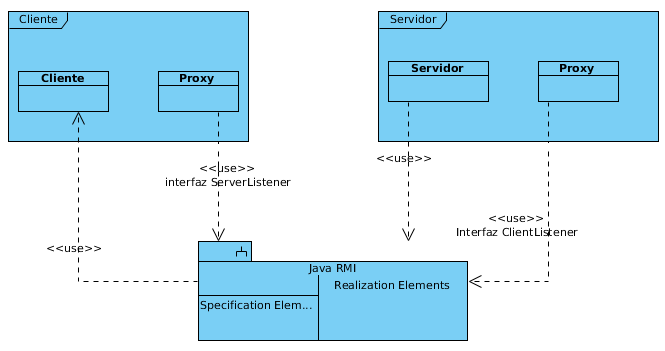
\includegraphics[scale=0.65]{img/arquitectura/arquitectura.png}
 \caption{Arquitectura del sistema}
 \label{arq_sistema}
 \end{figure}

\subsection{Arquitectura del cliente}
 
En la Figura \ref{arq_cliente} se muestra la arquitectura del cliente. Se ha utilizado una arquitectura MVC.
Además, se incluye una capa de comunicación:

\begin{itemize}
 \item \emph{Presentación:} Contiene las clases de las ventanas que se muestran al usuario y las interfaces que implementan.
 \item \emph{Controlador:} Contiene la lógica de control. Se encarga de comunicar a la interfaz los cambios de estado de la
 capa de dominio y de modificar el estado del dominio atendiendo a los cambios en la interfaz del juego.
 \item \emph{Dominio:} Contiene toda la lógica del juego. La clase Tablero9x9 es la clase principal e implementa las reglas del 
 juego. Se utiliza el patrón fachada para obtener un punto de acceso único a la capa de dominio. La clase encargada de 
 esta abstracción es FTERD.
 \item \emph{Comunicación:} Contiene las clases que realizan la función de \emph{listener} como es el caso de la clase Cliente,
 y el proxy con el servidor. Estas clases solamente se encargan del envío de los respectivos mensajes al servidor o a la fachada
 del paquete de dominio.
\end{itemize}

 \begin{figure}[h]
 \centering
 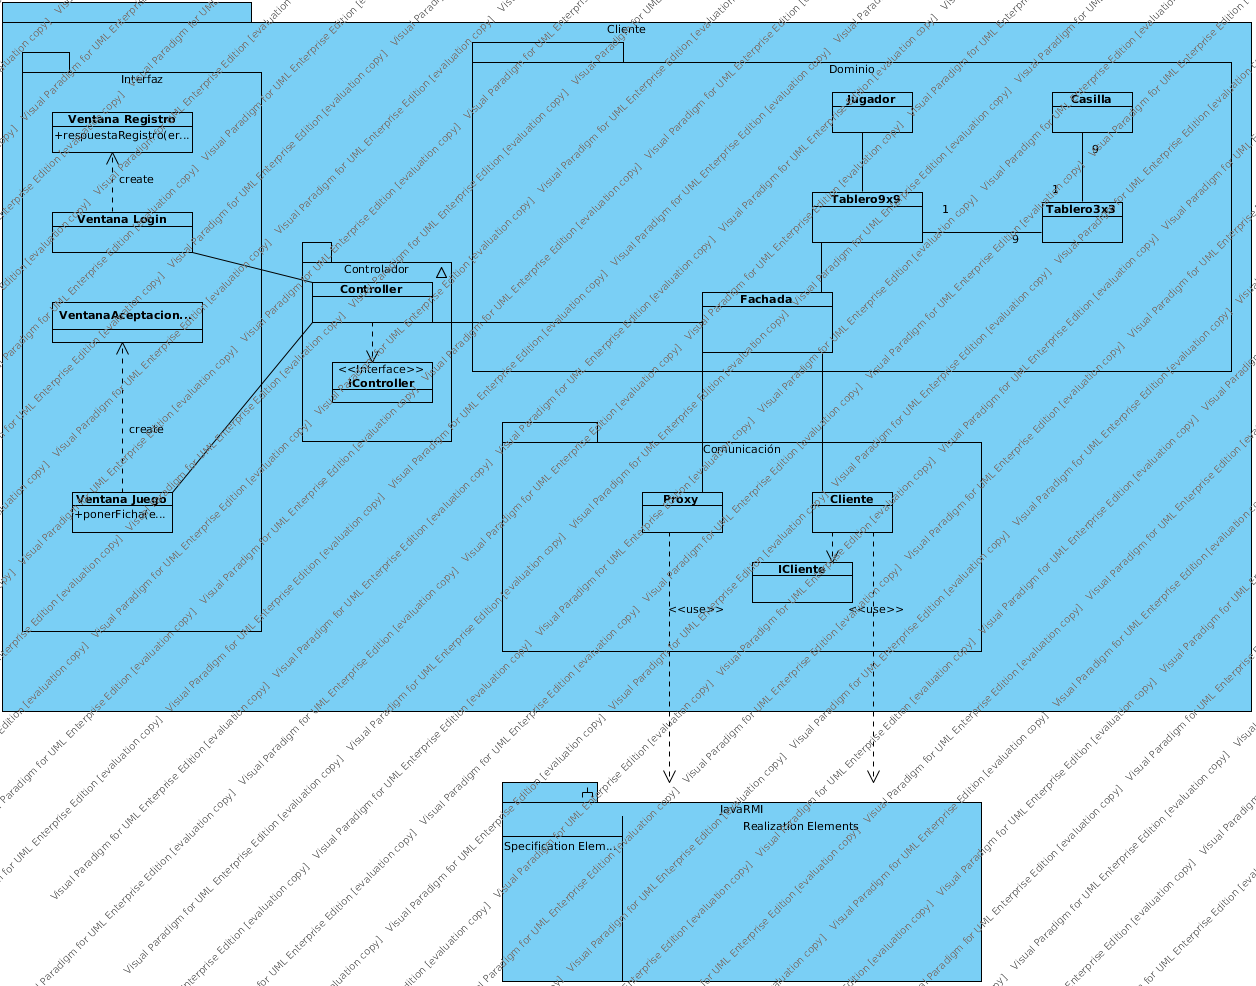
\includegraphics[scale=0.4]{img/arq_Cliente.png}
 \caption{Arquitectura del cliente}
 \label{arq_cliente}
 \end{figure}

\subsection{Arquitectura del servidor}

En la Figura \ref{arq_servidor} se muestra la arquitectura multicapa del servidor:

\begin{itemize}
 \item \emph{Comunicación:} Contiene las clases encargadas de la comunicación, en este caso la clase servidor y su interfaz
 RMI. La clase servidor actúa como \emph{listener} para escuchar solicitudes de los clientes. También responde a esos clientes,
 ya que internamente guarda una hash con los clientes que se han dado de alta en el sistema.
 \item \emph{Persistencia:} Contiene las clases encargadas de almacenar las partidas y sus respectivos tableros, jugadores
 y movimientos. Entre esas clases está la base \emph{Broker}, que actúa como agente entre el subsistema de base de datos y
 el sistema del servidor. Se ha optado por utilizar un patrón de fabricación pura en lugar de seguir el patrón experto para
 la persistencia. De esta forma, un conjunto de clases \emph{DAO} especializadas se encargan de almacenar los diferentes
 aspectos del dominio.
 \item \emph{Dominio:} Contiene las clases de dominio como las encargadas de representar a cualquier juego, además de la
 clase Fachada. Esta clase contiene una referencia a cada uno de los modelos que se están jugando en el sistema, es decir,
 contiene todos los tableros activos.
\end{itemize}


 \begin{figure}[h]
 \centering
 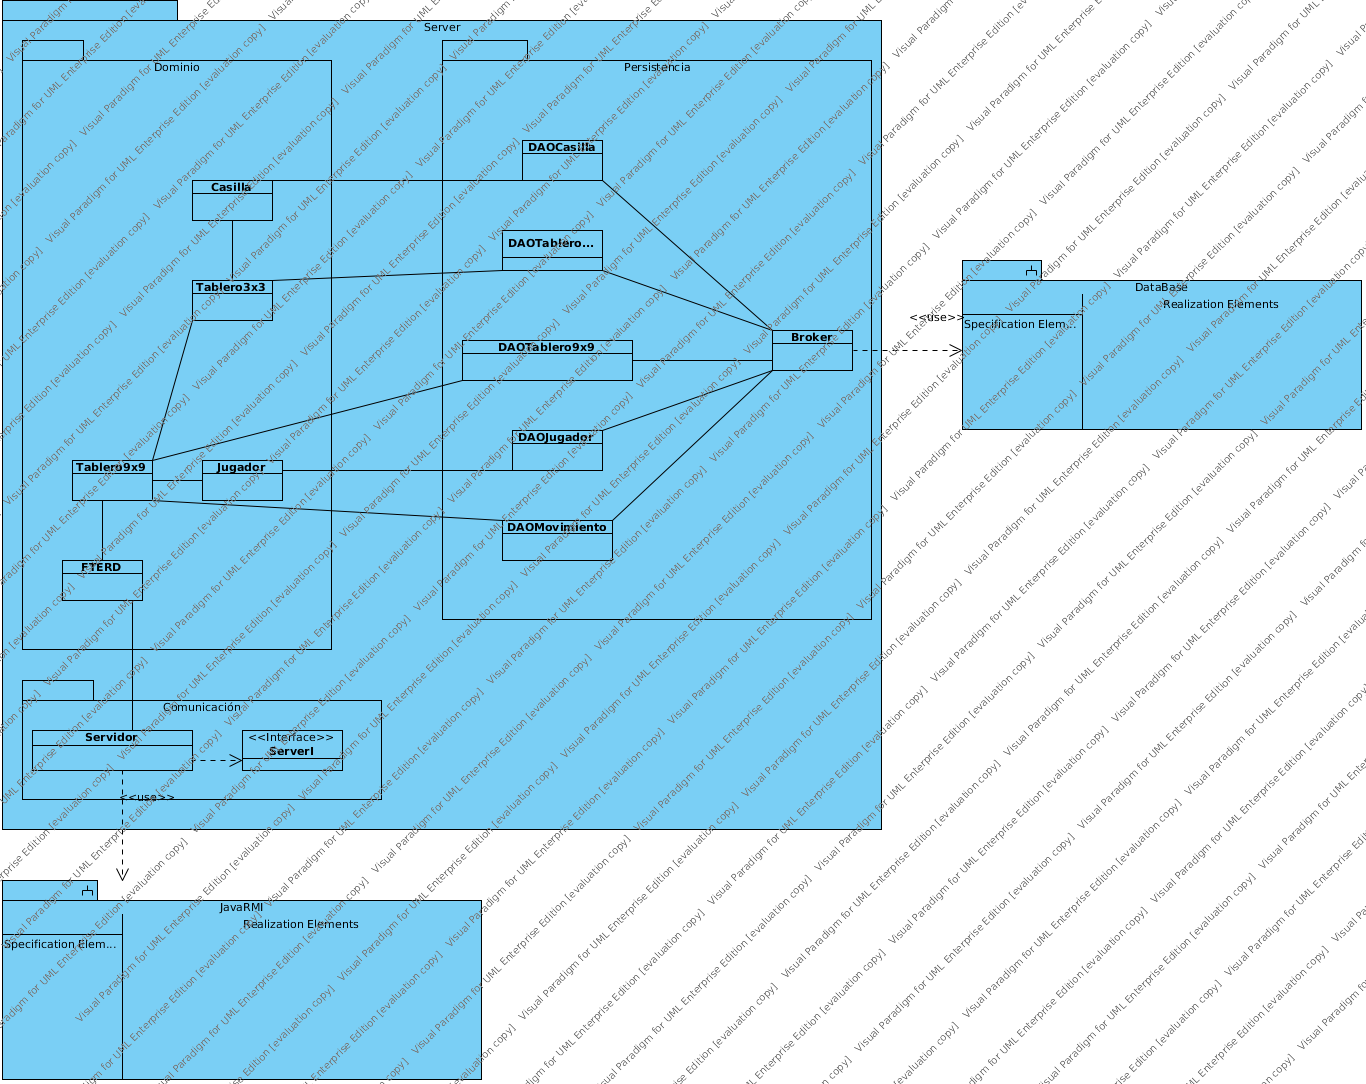
\includegraphics[scale=0.4]{img/arq_Servidor.png}
 \caption{Arquitectura del servidor}
 \label{arq_servidor}
 \end{figure}
 
\clearpage

\section{Pruebas de los casos de uso}

\subsection{Pruebas para la aplicación web}

Los test de la aplicación web han sido llevado a cabo mediante el testbed \emph{Selenium}. Las pruebas que han podido ser cubiertas y reproducibles han sido:

\begin{itemize}
\item Pruebas relacionadas con el login, posibles causas de error y de éxito.
\item Pruebas relacionadas con el registro, posibles causas de error y de éxito.
\item Pruebas relacionadas con el cierre de sesión, posibles causas de error y de éxito.
\end{itemize}

Para poder realizar estas pruebas ha sido necesario introducir una clase \emph{Broker} para la comunicación con la base de datos y una clase auxiliar que contiene las operaciones de borrado de esta base de datos.

Las pruebas relacionadas con la lógica de dominio por parte del cliente quedan cubiertas con las pruebas que se realizaron para el cliente web, ya que el código se ha cogido tal cual de esa implementación.

Se ha intentado realizar una prueba respecto de la jugabilidad, pero al no ser reproducible, se ha descartado. Estas pruebas han sido llevadas a cabo de forma manual con mucha dedicación y esfuerzo, probando las múltiples posibilidades para poder llevar la cobertura al máximo posible.

Las pruebas se encuentran en el paquete \emph{test.terd.web}.

\clearpage

\end{document}
